\newpage
\section{Module Interfacing and Robot Arm Programming}
Hye The d fmdodule for interfacing and programming the robot arm in \texttt{ABB RobotStudio®} involved establishing bidirectional communication between \texttt{MATLAB} and the robot controller to enable efficient pick and place operations. The \texttt{RAPID} programming language was employed to develop the robot program, allowing it to receive real-time instructions from \texttt{MATLAB} based on object properties identified through image processing.

\subsection{Communication Setup:}
Interfacing of \texttt{MATLAB} and \texttt{RobotStudio} in Client/Server Communication: \\ 
\noindent \textbf{\texttt{MATLAB} (Client):} \\
\texttt{MATLAB} is responsible for performing image processing and identifying the properties of the objects to be manipulated. It sends the coordinates, rotation angles, and properties of these objects to the robot controller over a socket connection. \texttt{MATLAB} also receives acknowledgment messages from the robot controller to confirm that the data has been received and processed correctly. \\
\noindent \textbf{\texttt{ABB RobotStudio} (Server):} \\
The robot controller, programmed in \texttt{RAPID} within \texttt{RobotStudio}, acts as the server in this setup. It listens for incoming connections from \texttt{MATLAB} and receives data strings representing the objects' properties.

\begin{figure}[H]
    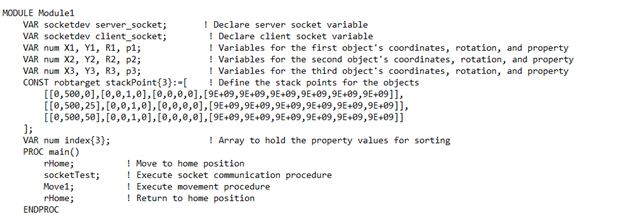
\includegraphics[width=7.4in ]{pics/abbstud.png}
    \label{abrrr}
\end{figure}

\textbf{Main Procedure (\texttt{main()}):} \\
The main procedure \texttt{main()} first calls \texttt{rHome()} to move the robot arm to the home position. It then executes the \texttt{socketTest()} procedure to establish the communication and receive data from \texttt{MATLAB}. Once the data is received, it is stored in an array (\texttt{index}) for sorting based on the properties of the objects.

The robot program begins with the declaration of server and client socket variables (\texttt{server\_socket} and \texttt{ client\_socket}). These sockets are essential for establishing the communication link between \texttt{MATLAB} and the \texttt{ABB} robot system. \texttt{MATLAB} acts as the client, sending data to the robot controller, which operates as the server, receiving and processing the data to execute the desired pick and place operations.

The \texttt{socketTest()} procedure handles the entire socket communication process. Initially, the server socket is created and configured with the \texttt{SocketCreate} and \texttt{SocketBind} commands. The server listens for incoming connections using \texttt{SocketListen}, and once a connection is accepted, \texttt{SocketAccept} establishes the communication link between the server and the client socket.


MATLAB sends data strings, which are received by the robot system using the SocketReceive function. These strings represent coordinates and properties of objects that need to be manipulated. The received data is converted from string format to numerical values using the StrToVal function and stored in predefined variables (X1, Y1, R1, p1) for each bar. After receiving and converting the data, the robot sends back acknowledgment messages to MATLAB using the SocketSend function.

\begin{center}
pickTargets{1}.trans := [X1, Y1, 0]; pickTargets{1}.rot := OrientZYX(R1, 0, 180); \\
pickTargets{2}.trans := [X2, Y2, 0]; pickTargets{2}.rot := OrientZYX(R2, 0, 180); \\
pickTargets{3}.trans := [X3, Y3, 0]; pickTargets{3}.rot := OrientZYX(R3, 0, 180); 
\end{center}



This part initializes the pickTargets array with the coordinates and rotations of the three bars. Each pickTargets element corresponds to a bar, with its position (trans) and orientation (rot) defined based on the received X, Y, and R values.

\begin{figure}[H]
    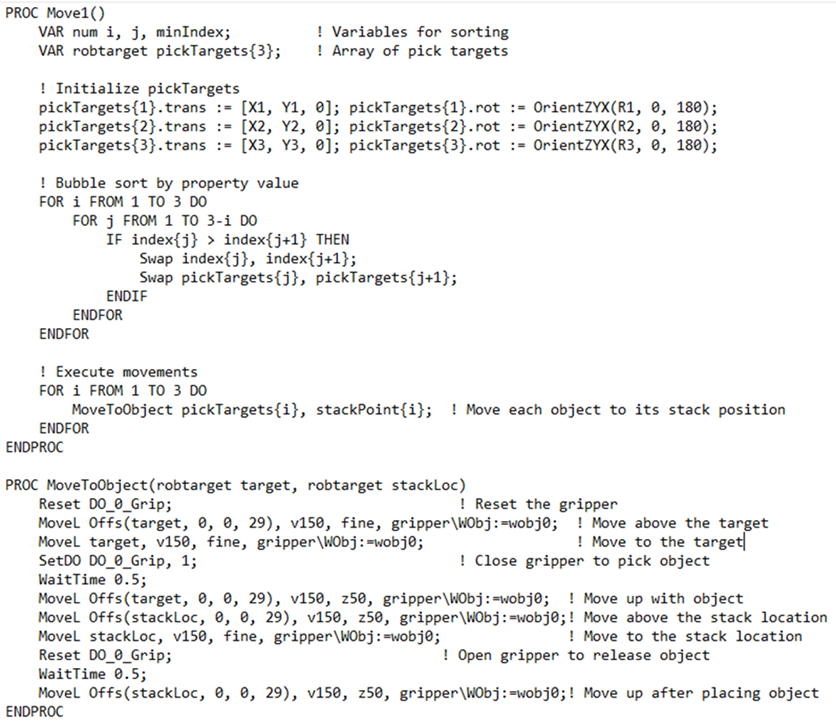
\includegraphics[width=5.5in ]{pics/PICKtARG.png}
    \label{PICK}
\end{figure}

\subsection{Movement and Sorting:}
In the \texttt{Move1} procedure, a bubble sort algorithm sorts the objects based on their properties. The sorted coordinates are then used to move the robot to each object's position. The \texttt{MoveToObject} procedure performs detailed pick and place actions, including moving to the object's location, gripping it, and placing it at the specified stack point. This involves precise movements defined by the \texttt{MoveL} commands, ensuring accurate positioning and manipulation of the objects within the workspace. The robot returns to the home position after completing the operations.

The \texttt{Move1()} procedure performs a bubble sort on the properties of the objects. This ensures that the objects are manipulated in the desired order. After sorting, the \texttt{MoveToObject()} procedure is called for each object to move it to its designated stack position. 

The \texttt{Move1()} procedure is central to the operation, handling the sorting of objects based on their properties and subsequently moving them to their designated stack positions. The procedure begins by implementing a bubble sort algorithm to arrange the objects. This sorting process utilizes a nested \texttt{FOR} loop, where the outer loop runs from 1 to 2, ensuring all elements are compared, and the inner loop runs from 1 to 3-i, facilitating the comparison of adjacent elements.

During each iteration of the inner loop, the property values of the current object (stored in the \texttt{index} array) are compared with the next object. If the current object's property value (\texttt{index\{j\}}) is greater than that of the next object (\texttt{index\{j+1\}}), a swap operation is initiated. This involves interchanging the elements within the \texttt{stackPoint} array, which holds the positions of the objects, to reflect the correct order. Additionally, the \texttt{Swap()} function is invoked to exchange the property values in the \texttt{index} array, ensuring both arrays remain synchronized.

Following the sorting process, the procedure proceeds to execute the movements of the objects. A \texttt{FOR} loop runs from 1 to 3, corresponding to the number of objects to be moved. Within this loop, the \texttt{MoveToObject()} procedure is called for each sorted position in the \texttt{stackPoint} array. This method ensures that each object is moved to its accurately sorted stack position, completing the sequence of operations. By utilizing the bubble sort algorithm and systematically calling the \texttt{MoveToObject()} procedure, the \texttt{Move1()} procedure ensures precise and efficient handling of the objects, fulfilling the requirements of the pick-and-place task.

The \texttt{MoveToObject()} procedure handles the detailed movements of the robot arm. It moves the arm to a position above the object, grips the object, lifts it, and places it in the designated stack position. This is achieved through a sequence of \texttt{MoveL} commands, ensuring smooth and precise movements. The \texttt{Reset DO\_0\_Grip} and \texttt{SetDO DO\_0\_Grip, 1} commands control the gripper to hold and release the objects appropriately.

Finally, after completing the pick and place operations, the \texttt{rHome()} procedure returns the robot arm to its initial home position, ensuring a safe and organized conclusion to the task. The robot controller processes the received data, converts it to numerical values, and uses this information to execute the pick and place operations. After processing the data, the robot sends acknowledgment messages back to MATLAB to confirm successful communication and execution.

\begin{figure}[H]
    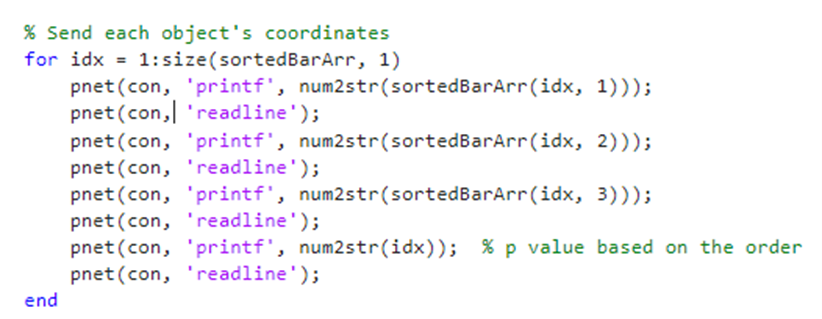
\includegraphics[width=4.5in ]{pics/MVOE.png}
    \label{PIC}
\end{figure}

\subsection{Data Transmission:}
The data sent between \texttt{MATLAB} and the \texttt{RAPID} program consists of the bar coordinates (\texttt{X}, \texttt{Y}), rotation (\texttt{R}), and a property value (\texttt{p}). The communication follows these steps:
\begin{enumerate}
    \item \texttt{MATLAB} establishes a TCP/IP socket connection to the robot controller.
    \item \texttt{MATLAB} sends the \texttt{X} coordinate of the first bar.
    \item \texttt{RAPID} receives the \texttt{X} coordinate and sends an acknowledgment back to \texttt{MATLAB}.
    \item \texttt{MATLAB} sends the \texttt{Y} coordinate of the first bar.
    \item It is repeated for the \texttt{R} and \texttt{p} values of the first bar and continues for the subsequent bars.
    \item After receiving all coordinates, the \texttt{RAPID} program processes the data for pick and place operations.
\end{enumerate}

